\section{Introduction}
\begin{frame}
\frametitle{Présentation du sujet}
\begin{center}
\begin{itemize}
\item Programmation sur un drone
\item Réalisation d'un jeu mobile
\item Architecture client-serveur
\end{itemize}
\begin{figure}
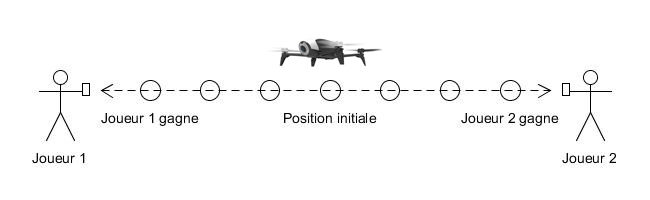
\includegraphics[scale=0.4]{images/partie.jpg}
\end{figure}
\end{center}

\textbf{BUT :} Contrôle à distance du drone

$\implies$ Démonstration publique à la \textit{Fête de la Science}
\end{frame}

\begin{frame}
\frametitle{Les outils}
\begin{center}
\begin{tabular}{p{5.5cm}p{5.5cm}}
\centering{DRONE PARROT BEBOP 2}  & \centering{ANDROID SDK} \tabularnewline
\centering{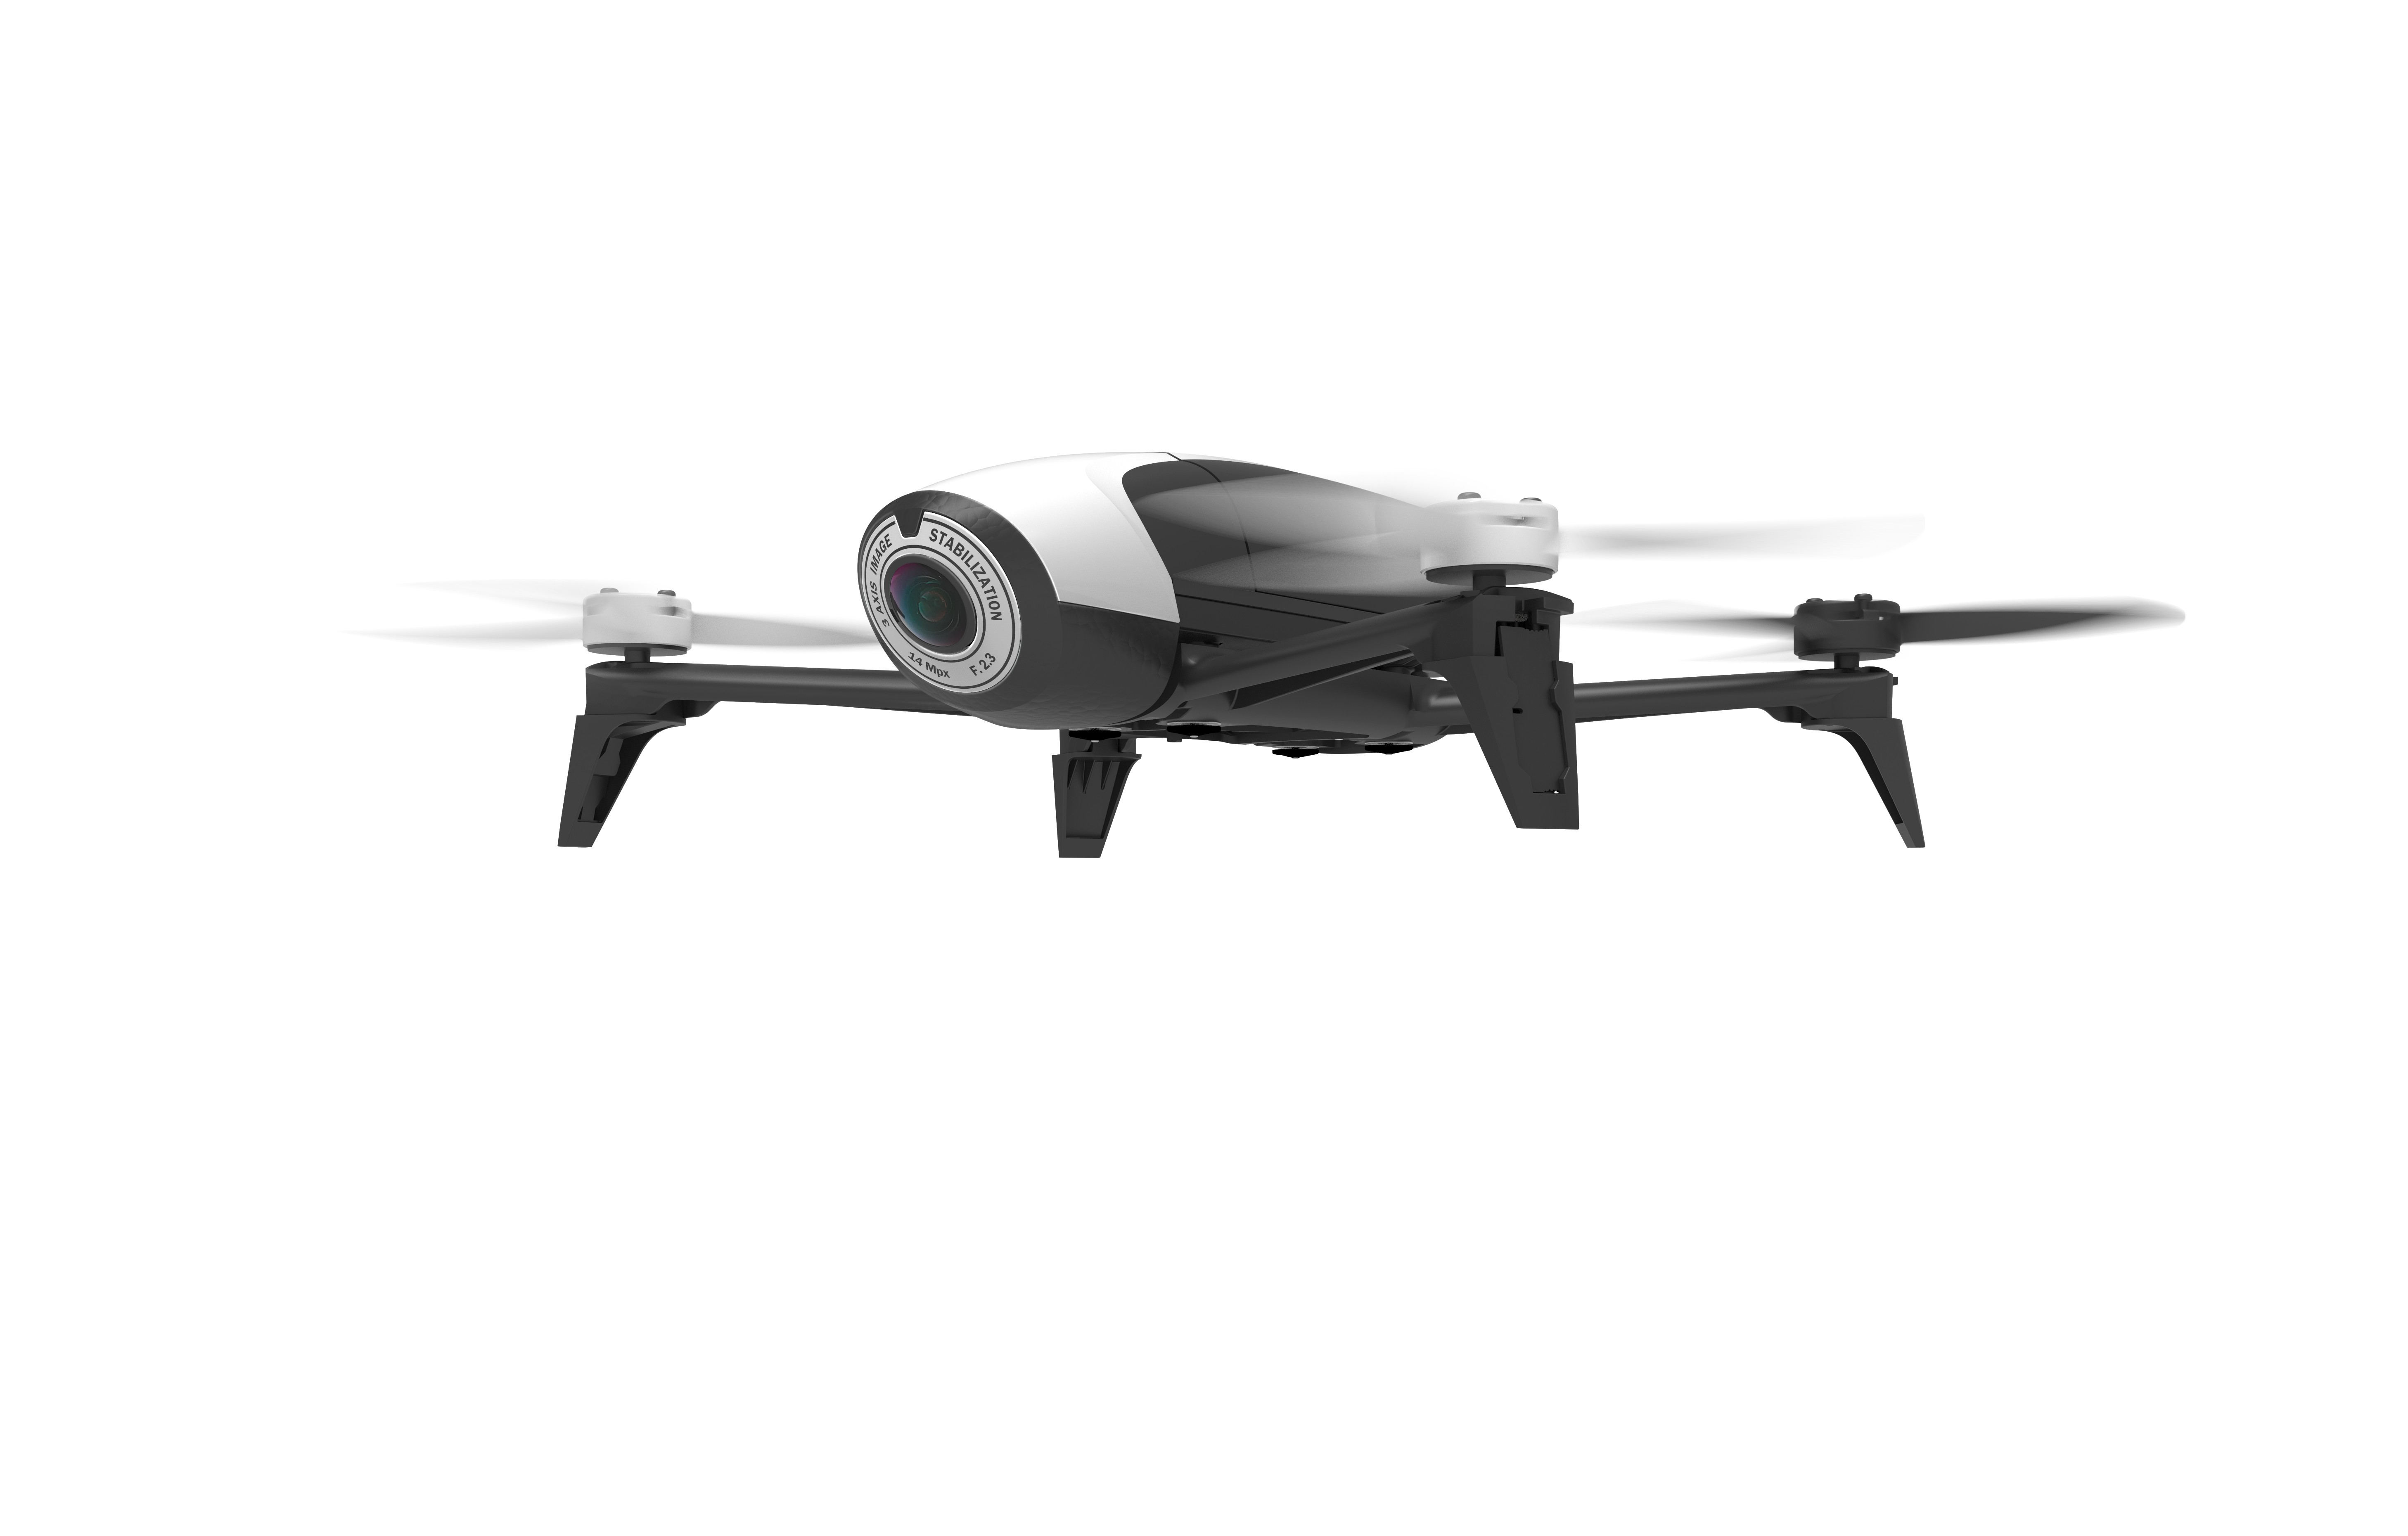
\includegraphics[scale=0.02]{images/drone.jpg}}  & \centering{
\includegraphics[scale=0.2]{images/android.jpg}} \tabularnewline
poids : 500g & \centering Java \tabularnewline
autonomie : 25min & \centering frameword \textit{libGDX} \tabularnewline
antenne Wi-Fi jusqu'à 300m & \tabularnewline
Application \textit{Free Flight Pro} & \tabularnewline
\end{tabular}
\end{center}
\end{frame}